\begin{figure}
	\centering
	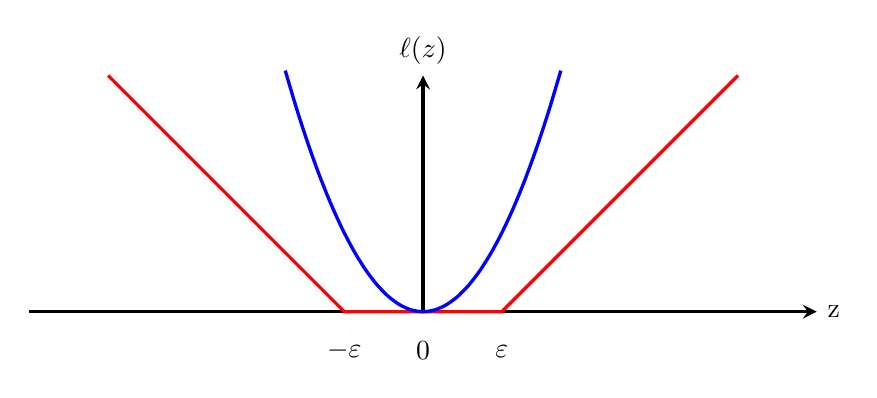
\begin{tikzpicture}
    
		\draw[very thick,-stealth] (-5,0) -- (5,0) node[right] {z};
		\draw[very thick,-stealth] (0,0) -- (0,3) node[above] {$\ell(z)$};

		\draw[red,very thick] (-4,3) -- (-1,0) -- (1,0) -- (4,3);
		\draw[domain=-1.75:1.75,smooth,variable=\x,blue,very thick] plot ({\x},{\x*\x});

		\node at (-1,-0.5) {$-\varepsilon$};
		\node at (1,-0.5) {$\varepsilon$};
		\node at (0,-0.5) {0};
		
	\end{tikzpicture}
\end{figure}